% !TEX TS-program = xelatex


\documentclass[a4paper,14pt]{extarticle}

% Include settings from setting.tex
\input{setting.tex}

\geometry{a4paper, margin=1in}
\graphicspath{{img/}}

\newcommand{\assignNum}{4} %change the number of the assignment here
\author{مرتضی ملکی‌نژاد شوشتری} %change your name here
\newcommand{\SNum}{810104256} %change your SID here
\date{\today}
\title{تمرین \assignNum}

\begin{document}
\pagenumbering{gobble}
\maketitle
\newpage
\tableofcontents

\newpage
\listoffigures

\newpage
\listoftables

\newpage
\pagenumbering{arabic}

\section{چکیده}

\newpage
\setcounterref{section}{0}

\lr{\section{Convergence of K-means}}
\lr{\subsection{a}}
\begin{itemize}
\item 
حتی با یک 
\lr{tie braking}
که 
\lr{deterministic}
نیست هم، مقدار فاصله درون خوشه‌ای زیاد نمی‌شود. اما 
\lr{deterministic}
نبودن باعث می‌شود تا فاصله درون خوشه‌ای بهبود نیابد، جواب قابل دستیابی دوباره نباشد، بهترین جواب بدست نیاید و یا خوشه‌بندی بیشتر طول بکشد. ولی اگر معیار توقف روی عدم بهبود فاصله درون خوشه‌ای باشد، الگوریتم حتما پایان می‌پذیرد. اگر معیار پایان الگوریتم، عدم تغییر خوشه‌ها باشد ولی ممکن است که پایان نیابد. در شکل 
\ref{q1_1}
مثالی از این مورد زده شده است.
{
\centering
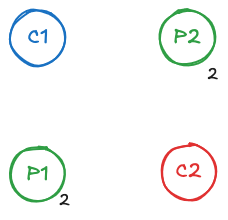
\includegraphics[width=0.4\textwidth]{img/q1.png}
\label{q1_1}
\tiny
\captionof{figure}{در \lr{p1} و \lr{p2} هرکدام دو نقطه وجود دارد (یعنی در کل شش نقطه موجود است). اگر هرکدام از آن‌ها یکبار به \lr{c1} و یکبار به \lr{c2} متعلق شوند، خوشه‌بندی ممکن است هیچوقت تمام نشود. }
}
\item 
اگر کلاس با پایین ترین شماره اساین شود هیچوقت نوسان کلاس رخ نمی‌دهد. حال تنها چیزی که باید ثابت شود این است که تابع 
\lr{F}
همواره غیر صعودی است. هدف 
\lr{F}
درواقع یافتن مقادیر \lr{c} است به طوری که مقدار  زیر کمینه شود:
\begin{latin}
	~\\
	$
	F = \sum \sum || (x - c_i)^2 || 
	$
\end{latin}
اگر فقط برای یک خوشه درنظر بگیریم:
\begin{latin}
	~\\
	$
	w = \sum (x - c_i)^2 \xrightarrow{derviative} \sum 2(x - c_i ) = 0 \Rightarrow n c_i = n \bar{x} \Rightarrow c_i = \bar{x}
	$
\end{latin}
یعنی میانگین هر خوشه، فاصله درون خوشه‌ای را کمینه می‌کند. و چون این میانگین معیار تشخیص مرکز جدید در
\lr{KNN}
است پس همواره رو به کم شدن می‌رود. پس هیچوقت زیاد نمی‌شود.
\end{itemize}
\lr{\subsection{b}}
\begin{itemize}
	\item 
	چون خوشه هیچ عضوی ندارد، نمی‌توان مرکز خوشه را حساب کرد. 
	\item 
	می‌توان نقطه‌ای که از مرکز خوشه‌ها بیشترین فاصله را دارد به عنوان مرکز خوشه جدید درنظر گرفت. 
	\item 
	بله. می‌توان با استفرا ثابت کرد که پس از انتخاب مرکز خوشه جدید فاصله حتما کاهش می‌یابد. به ازای هر نقطه،‌اگر در حالتی که مرکز جدید نبود فاصله آن با نزدیکترین مرکز 
	$d_i$ 
	بوده، همچنان این مرکز موجود است و نقطه اگر به مرکز جدید نباشد، همچنان باعث می‌شود مقدار $d_i$  به فاصله درون خوشه‌ای اضافه شود و نه بیشتر. ولی نقطه‌ای که به تازگی مرکز خوشه شده است، فاصله درون خوشه‌ای آن صفر می‌شود. پس یعنی فاصله درون خوشه‌ای در حالت کل کمتر می‌شود.
\end{itemize}
\newpage
\lr{\section{Regularized K-Means and MAP Estimation}}
\lr{\subsection{a}}
\begin{enumerate}
	\item 
	داریم:
	\begin{latin}
		~\\
		$
		J = \sum (x_j - \mu_i)^2 + \lambda \mu_i^2 \xrightarrow{derviative} \sum 2( \mu_i - x_j) + 2 \lambda \mu_j  \Rightarrow n \mu_j - n \bar{x} + \lambda \mu_j = 0
		\Rightarrow \mu_j = \cfrac{n\bar{x}}{n + \lambda}
		$
	\end{latin}
	\item 
	اگر مقدار 
	$\lambda$
	خیلی کوچک باشد، عملا 
	\lr{Regularization}
	ای نداریم و همان میانگین گروه درنظر گرفته می‌شود. و اگر این مقدار بسیار بزرگ باشد، میانگین ها به صفر نزدیک می‌شوند.
	
\end{enumerate}
\lr{\subsection{b}}
\begin{enumerate}
	\item 
	برای این کار اول باید جمع را به ضرب تبدیل کرد. در 
	\lr{MAP}
	با گرفتن لگاریتم ضرب به جمع تبدیل می‌شود پس اینجا باید برعکس آنکار را کرد (و چون هم لگاریتم و هم توان رساندن رابطه یکنوا و صعودی هستند، بیشینه کردن هر دوعبارت یکسان است.) پس داریم:
	\begin{latin}
		~\\
		$
		(\prod e^{(x_j - \theta)^2} ) e^{\lambda(\theta^2)}
		$
	\end{latin}
	\item 
	برای 
	\lr{posterior}
	باید توزیع با پارامتر 
	$\theta$
	ای را پیدا کرد که تتا فقط در عبارت 
	$e^{(x - \theta)^2}$
	تاثیر داشته باشد. برای مثال توزیع نرمال با واریانس یک همچنین ویژگی‌ای دارد. 
	
	 توزیع 
	\lr{prior}
	نیز شبیه یک توزیع  نرمال است که واریانس آن برابر با 
	$\cfrac{1}{\lambda}$
	. پس یعنی اگر ضرایب ثابت درنظر گرفته نشوند، مقداری که سعی در بهینه کردن آن داریم معادل یک 
	\lr{MAP}
	است که در آن توزیع 
	\lr{prior}
	یک توزیع نرمال با واریانس 
	$\cfrac{1}{\lambda}$
	 است و توزیع 
	\lr{likelihood}
	یک توزیع نرمال با واریانس یک است.
	\item 
	باتوجه به قسمت قبل داریم:
	\begin{latin}
		$
		P_N(0, \sigma) = e^{\frac{x^2}{\sigma^2}} = e^{\lambda x^2} \Rightarrow \lambda \sigma^2 = 1 \Rightarrow \sigma^2 = \frac{1}{\lambda}
		$
	\end{latin}
\end{enumerate}
\newpage
\lr{\section{The K-Means Objective Identity}}
اگر در عبارت اولیه یک 
$
\mu_i 
$ 
جمع و تفریق کنیم داریم:
\begin{latin}
	~\\
	$
	Z = \sum\limits_{l = 1}^k \cfrac{1}{2|C_l|} \sum\limits_{i,j \in C_l} || x_i - x_j || ^2
	= \sum\limits_{l = 1}^k \cfrac{1}{2|C_l|} \sum\limits_{i,j \in C_l} || x_i - \mu_l + \mu_l - x_j || ^2
	\\
	= \sum\limits_{l = 1}^k \cfrac{1}{2|C_l|} \sum\limits_{i,j \in C_l} (|| x_i -  \mu_l || ^2  + ||\mu_l - x_j || ^2  + 2( x_i -  \mu_l )( \mu_l - x_j))
	$
\end{latin}
واضح است که دوعبارت اول برابر می‌شوند با دوبرابر حاصل جمع حاصل تفاضل مقادیر از میانگین به توان دو پس داریم:
\begin{latin}
	~\\
	$
	Z = \sum\limits_{l = 1}^k  \sum\limits_{i \in C_l} ( \cfrac{|C_l| || x_i -  \mu_l || ^2}{{|C_l|}} ) +  \sum\limits_{l = 1}^k  \sum\limits_{i, j \in C_l} \cfrac{2}{{|C_l|}}( x_i -  \mu_l )( \mu_l - x_j)
	\\
	=  \sum\limits_{l = 1}^k  \sum\limits_{i \in C_l} (|| x_i -  \mu_l || ^2 ) +  \sum\limits_{l = 1}^k  \sum\limits_{i, C_l} \cfrac{2}{{|C_l|}}( x_i -  \mu_l ) \sum \limits_{j \in C_l} ( \mu_l - x_j)
	$
	
\end{latin}
واضح است که حاصل جمع آخرین سیگما صفر است پس داریم:
\begin{latin}
	~\\
	$
	Z =  \sum\limits_{l = 1}^k  \sum\limits_{i \in C_l} (|| x_i -  \mu_l || ^2 ) +  \sum\limits_{l = 1}^k  \sum\limits_{i, C_l} \cfrac{2}{{|C_l|}}( x_i -  \mu_l ) * 0
	 \sum\limits_{l = 1}^k  \sum\limits_{i \in C_l} (|| x_i -  \mu_l || ^2 ) +  0
	 \\
	 = \sum\limits_{l = 1}^k  \sum\limits_{i \in C_l} (|| x_i -  \mu_l || ^2) 
	$
\end{latin}
که این همان عبارت سوال است.
\newpage
\lr{\section{Gaussian Mixture Model}}
\lr{\subsection{A}}

\begin{table}[h]
	\centering
	\caption{ویژگی‌های انتخاب شده در هر دو روش}
		\begin{adjustbox}{width=\textwidth}
		\begin{tabular}{|c|c|c|}
			\hline
			\lr{Group} & \lr{method} & \lr{Reason}\\
			\hline
			\lr{A} & \lr{GMM} & این مدل نواحی بیضوی شکل دارد. عملا شبیه کانتورهای دو یا چند توزیع نرمال \\
			\lr{B} & \lr{KNN} & تصاویر عملا در گروه‌های دایره شکل قرار گرفته‌اند. این ویژگی knn است زیرا فاصله را از وسط حساب می‌کند و عملا نواحی به شکل دایره در می‌آیند. \\
			\lr{C} & \lr{Single Link} & در این مدل کمترین فاصله بین هر دو گروه متفاوت بیشینه شده است و این ویژگی این الگوریتم است. \\
			\hline
		\end{tabular}
		\end{adjustbox}
\end{table}
\lr{\subsection{B}}
اول باید 
\lr{likelhood}
هر نقطه حساب شود. و سپس 
\lr{MLE}
انجام شود با این تفاوت که وزن هر نقطه برابر با 
\lr{likelihood}
آن است که توسط جمع 
\lr{likelhood}
ها نرمالایز شده. با اجرای این کار به نتایج زیر میرسیم: (محاسبات در فایل \lr{2.ipynb} هستند.)
\begin{latin}
	~\\
	$
	\mu_1 = \begin{bmatrix}
		-0.239 \\
		0.965
	\end{bmatrix}
	\mu_2 = \begin{bmatrix}
		3.015 \\
		-0.343
	\end{bmatrix}
	\Sigma_1  = \begin{bmatrix}
		0.439 & -0.414 \\
		-0.414 & 0.679
	\end{bmatrix}
	\Sigma_2  = \begin{bmatrix}
		0.726 & -0.347 \\
		-0.347 & 0.230
	\end{bmatrix}
	$
\end{latin}
اگر مقدار 
\lr{likelhood}
را برای هر خوشه حساب کنیم داریم:
\begin{latin}
	~\\
	$
	L_1 \approx 0.0063 \quad L_2 \approx 0.0147 
	$
\end{latin}
پس یعنی به خوشه دوم تعلق دارد.
\newpage
\lr{\section{EM}}
\lr{\subsection{a}}
اینجا 
باید بجای 
\lr{mle}
عملا 
\lr{map}
را انجام داد. توزیع بتا توزیع  
\lr{prior}
برای 
$\mu$
 است و توزیع دیریکله توزیع \lr{prior} برای 
 $\pi$
 است.
 \lr{\subsection{b}}
 در بخش 
 \lr{expectation}
 عملا تغییری رخ نمی‌دهد (چون \lr{likelihood} حساب می‌شود و سعی در تخمین چیزی نیست.)
 پس داریم:
 \begin{latin}
 	$
 	w_{ik} = \cfrac{\pi_k P(x_i | \mu_k)}{\sum \limits_{j = 1}^{K} \pi_j P(x_i | \mu_j)}
 	=  \cfrac{\pi_k \mu_k^{x_i} (1 - \mu_k)^{1 - x_i}}{\sum \limits_{j = 1}^{K} \pi_j \mu_k^{x_i} (1 - \mu_k)^{1 - x_i}}
 	$
 \end{latin}
 \lr{\subsection{c}}
 توزیع بتا به عنوان 
 \lr{prior}
 این نقش را عمل می‌کند که به داده‌های مشاهده شده، 
 $a$
 موفق و 
 $b$
 ناموفق اضافه شود. همچنین فرض توزیع دیریکله برای 
 \lr{prior}
 بخش 
 $\pi$
 باعث می‌شود تا بجای محاسبه 
 $\pi$
 فقط براساس وزن، مقدار 
 $\alpha_i$
 را به آن اضافه کرد. اگر 
 \lr{prior}
 نبود داشتیم:
 
\begin{latin}
	~\\
	$
	\mu_i = \sum_{j  = 1}^n \cfrac{w_{ij}}{total\ weight} x_i = \cfrac{ \sum_{j  = 1}^n w_{ij} x_i }{total\ weight}
	$
\end{latin}
ولی با احتساب داده‌های فرض شده از توزیع بتا داریم:
\begin{latin}
	~\\
	$
	\mu_i = \cfrac{ \sum_{j  = 1}^n w_{ij} x_i + a - 1 }{total\ weight + a + b - 2}
	$
\end{latin}
بطور مشابه برای توزیع دیریکله داریم:
\begin{latin}
	~\\
	$
	\text{no prior} \Rightarrow \pi_i = \cfrac{\sum\limits_{j = 1}^n w_{ij}}{\sum\limits_{w = 1}^K \sum\limits_{j = 1}^n w_{wj}}
	\\\\
	\text{ prior} \Rightarrow \pi_i = \cfrac{\sum\limits_{j = 1}^n w_{ij} + \alpha_i}{\sum\limits_{w = 1}^K (\alpha_w +  \sum\limits_{j = 1}^n w_{wj})}
	$
\end{latin}

\end{document}